\chapter{Background}

In this chapter, we go through the theory of methods which are used in the work.

%----------------------------------------------------------------------
\section{\todo{History of machine translation}}

\todo{rephrase \cite{Han2016}}


%----------------------------------------------------------------------
\section{\todo{Transformer model}}

Introduced in \perscite{vaswani-2017-transformer} Transformer model is used as a base
for numerous state-of-the-art systems as can be seen for example in 
WMT18 \parcite{bojar-etal-2018-findings} and
WMT19 \parcite{barrault-EtAl:2019:WMT} results.

Prior to invention of the \textit{Transformer} model, \acrfull{rnn} and \acrfull{cnn}
architectures were used
to encode source side of the sentence pair and to decode it into the target sentence.
Various window lengths in \acrshort{cnn} architectures allowed to capture
long range relations as well as short range ones;
still the range was limited by the maximum window length.
In \acrshort{rnn}-like architectures \acrfull{lstm} and \acrfull{gru} cells
were used, as their structure allowed to pass the internal state
on longer distances due to selective forgetting.

\textit{Transformer} model uses the \textit{self attention} mechanism
to encode contextual information in each word position.
\textit{Position encoding} allows passing the position
information without explicit sequential connections as in \acrshort{rnn}.
Architecture of the \textit{Transformer} model is shown
on \cref{fig:transformer_architecture}.
For tasks involving very long sequences autors also proposed \textit{restricted}
self-attention, which considers only a neighborhood of size $r$ in the input
sequence centered around the respective output position.
As was stated by \textit{Transformer}'s authors, there are three main points why
self-attention mechanism should be preferred
(which are compared with \acrshort{rnn} and \acrshort{cnn}
in \cref{tab:layer_complexity_comp}):
\begin{itemize}
  \item total computational complexity per layer;
  \item the amount of computation that can be parallelized;
  \item the path length between long-range dependencies in the network.
\end{itemize}

\begin{table}
\centering
\begin{tabular}{l|ccc}
\toprule
Layer type        &   Complexity             &  Sequential & Maximum        \\
                  &   per layer              &  operations & path length    \\
\midrule
Self-Attention    & $O(n^2 \cdot d)$         & $O(1)$      & $O(1)$         \\
Recurrent         & $O(n \cdot d^2)$         & $O(n)$      & $O(n)$         \\
Convolutional     & $O(k \cdot n \cdot d^2)$ & $O(1)$      & $O(log_k (n))$ \\
Self-Attention (restricted) & $O(r \cdot n \cdot d)$       & $O(1)$ & $O(n/r)$  \\
\bottomrule
\end{tabular}
\mycaption{Maximum path lengths, per-layer complexity and minimum number of sequential operations for different layer types} {
	$n$ is the sequence length, 
	$d$ is the representation dimension, 
	$k$ is the kernel size of convolutions and 
	$r$ the size of the neighborhood in restricted self-attention.
}
\label{tab:layer_complexity_comp}
\end{table}


\begin{figure}[h]
	\centering
	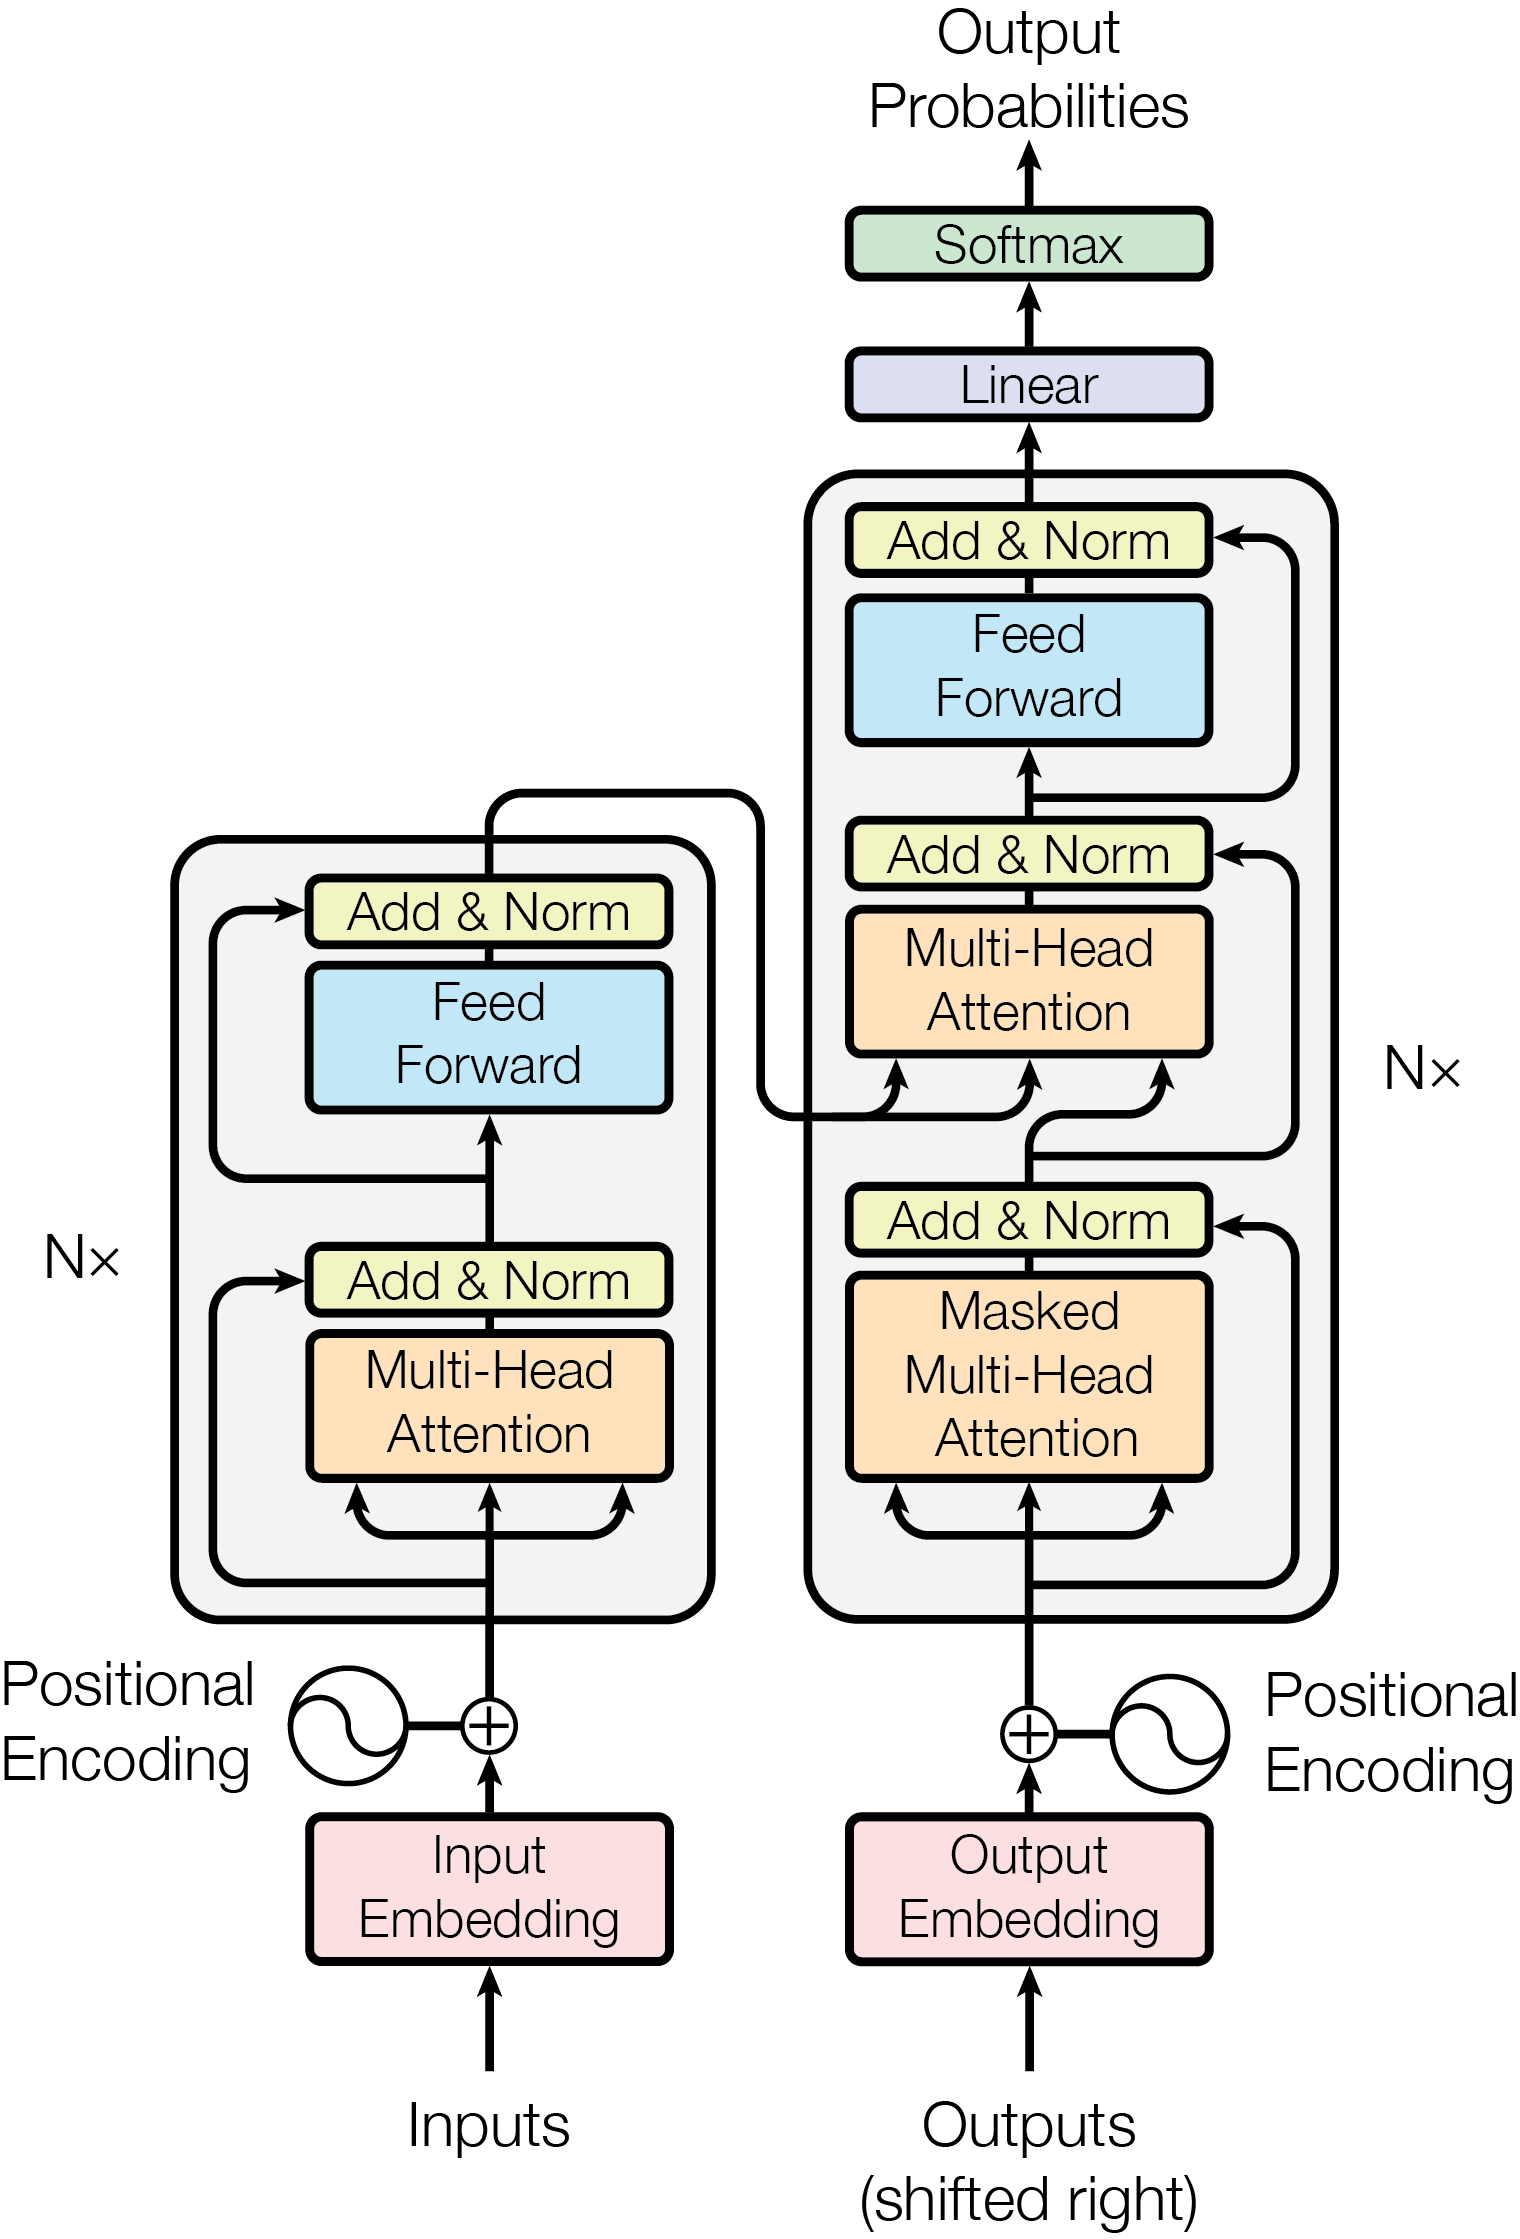
\includegraphics[width=0.9\columnwidth]{../img/transformer_architecture.png}
	\mycaption{Transformer model architecture} {}
	\label{fig:transformer_architecture}
\end{figure}


%----------------------------------------------------------------------
\section{\todo{Preprocessing: BPE}}
\label{section:bpe}
\todo{models for the big UN corpus were trained with SentencePiece, not BPE}

%----------------------------------------------------------------------
\section{Translation evaluation}

\subsection{History}

In 1966 first machine translation evaluation methods were proposed
by the \acrfull{alpac}.
The proposed metrics were ``intelligibility" and ``fidelity"
\citep[p~67]{Translation1966}.
Trained human raters were needed to measure the metrics.

Later, after years of using manual evaluation, automatical evaluation
metrics were created, such as word error rate (WER) \cite{Su1992},
translation edit rate (TER) \cite{Snover2006}, etc.
Nowadays the most popular metric is \acrfull{bleu} which is described
in the next section.


\subsection{BLEU - bilingual evaluation understudy}

In \cite{Papineni02bleu} a nowel method of automatic machine
translation evaluation was introduced - \acrfull{bleu}.
Its advantages are the high speed and low cost of evaluation,
language independence and high correlation with judgements
of highly skilled human raters.

Shortly, \acrshort{bleu} score consists of modified n-gram precision scores
corrected by brevity penalty,
which ensures the produced translation lenght is close to the reference one.
\acrshort{bleu} score is computed for the whole test corpus.

\subsubsection*{Modified \textit{n}-gram precision score}

The main element of the metric is the \textit{precision} measure.
It is computed in the following way:
the number of candidate translation words (unigrams) that are present in
any reference translation is divided by the total number of words in the candidate translation.
This approach leads to overrating candidate translation which consists of only one
or a couple of words that occur in reference translations, as can be seen in
\cref{exmp:precision-modified-1gram-precision}.

Intuitively, after a word from the reference translation has occurred,
it should not be considered in the calculation anymore.
This intuition is formalized as the \textit{modified unigram precision}.
It is computed in the following way:
\begin{enumerate}
	\item count the maximum number of occurrences of a word in any reference translation;
	\item clip the total count of every candidate word by the maximum reference count;
	\item sum the clipped counts;
	\item divide this sum by the total (not clipped) number of candidate words.
\end{enumerate}
As a result, the sentence which may receive a high precision score will receive
more realistic evaluation measured by modified precision score, as can be seen in
\cref{exmp:precision-modified-1gram-precision}.

\vspace{\baselineskip}
\begin{minipage}{0.9\textwidth}

	Candidate: \underline{of} \underline{of} \underline{of} of of of of of of of

	Reference: London is the capital \underline{of} England and \underline{of} the United Kingdom
	\underline{of} Great Britain and Northern Ireland.

	Precision: 10/10 = 1.0

	Modified unigram precision: 3/10 = 0.3

	\begin{exmp}
	Precision and modified unigram precision.
	Similarly is computed modified $n$-gram precision score for any $n$,
	but $n$-gram counts are collected instead.
	\label{exmp:precision-modified-1gram-precision}
	\end{exmp}

\end{minipage}
\vspace{\baselineskip}

\subsubsection*{Sentence length}

A produced translation should not be too short or too long.
It is usually done by pairing precision with \textit{recall}.
However, in \acrshort{bleu}, multiple reference sentences can be used
for one source sentence, so recalling all possible translations from
every reference is not what is needed.
\acrshort{bleu} authors introduced the \textit{brevity penalty} factor
for this purpose.
In short, it penalizes produced translations that are shorter than the references.
To avoid excessive penalization of shorter sentences,
the \textit{brevity penalty} is computed on the whole translated set.
In the equation below, $r$ is the test corpus’ effective reference length
and $c$ is the total length of the candidate translation corpus.
To compute $r$ the best match lengths for each candidate sentence
in the corpus are added.

\begin{equation}
\label{eq:brevity_penalty}
    BP=
    \begin{cases}
		1,           & \text{if } c > r;\\
		e^{1-r/c}, & \text{otherwise}
    \end{cases}
\end{equation}

\subsubsection*{Equation}

Combining all the above, the metric works in this way (\cref{eq:bleu}):
\begin{enumerate}
	\item compute the geometric mean of the modified
		n-gram precisions ($p_n$), using n-grams up to length $N$
		and positive weights ($w_n$) summing to one.
	\item compute \textit{brevity penalty} as in \cref{eq:brevity_penalty}.
	\item multiply results of steps 1. and 2.
\end{enumerate}
Authors proposed to use $N=4$ and uniform weights $w_i = 1/4$.

The metric value is in a range from 0 to 1.
However, popular implementations such as SacreBLEU \citep{Post2018-sacrebleu}
report it in percentage points from 0 to 100.


\begin{equation}
\label{eq:bleu}
	BLEU=BP \cdot \exp \left(\sum_{n=1}^{N} w_n \log p_n \right)
\end{equation}


%----------------------------------------------------------------------
\section{Multi-target machine translation}
\label{section:multitarget_mt}

In this section, we have a closer look at an area in \acrshort{mt},
which this thesis is dedicated to -- multi-target \acrshort{mt}.
First, we talk about multi-lingual \acrshort{mt} in general: multi-way,
multi-source and multi-target.
Later we describe the specific approach from multi-lingual \acrshort{mt}
-- complete sharing of model parameters, which we are using in this work.


\subsection{Multi-lingual machine translation}

With constant improvement of neural \acrshort{mt} systems performance,
researchers started to experiment with incorporating multiple source
languages, or target languages, or both, into one model,
and the results are promising:
\begin{itemize}
	\item having \dir{L1}{L2} and \dir{L2}{L3} non-parallel
	corpora allows to train a model that can produce \dir{L1}{L3} translation
	of decent quality \fix{cite some paper};
	\item having a high-resource L1 and low-resource L2
	from the same language group helps increase \dir{Source}{L2} translation
	quality with pretraining on \dir{Source}{L1} data \fix{cite the paper}.
\end{itemize}

Even if the concept of combining multiple languages into one model and possible outcomes
of such combination may seem intuitive, there exist multiple approaches of how exactly
this might be performed. As for current time, \cite{Dabre2019} categorizes
MNMT (multi-lingual neural machine translation) in the following way
(Figure \ref{fig:mnmt_categorized}):

\textbf{Multi-Way Translation.}
The goal is constructing a single \acrshort{nmt} system for
one-to-many, many-to-one or many-to-many
translation using parallel corpora for more than one language pair.

\textbf{Low or Zero-Resource Translation.}
Large amounts of parallel texts of high quality are available for most of European
languages. However, it is not true for most of other languages in the world.
Three main directions have been studied for these cases.
\textit{Transfer learning}: Transferring translation knowledge from a high-resource language pair
to improve the translation of a low-resource language pair.
\textit{Pivot translation}: Using a high-resource language (usually English) as a pivot to translate
between a language pair.
\textit{Zero-shot translation}: Translating between language pairs without parallel corpora.

\textbf{Multi-Source Translation.} Having the source side represented by multiple languages
may increase translation quality in general or help to remove ambiguities present in one or another
source language (e.g. cases, noun genders, etc.).


\begin{figure}[h]
	\begin{minipage}{0.9\textwidth}
	\centering
	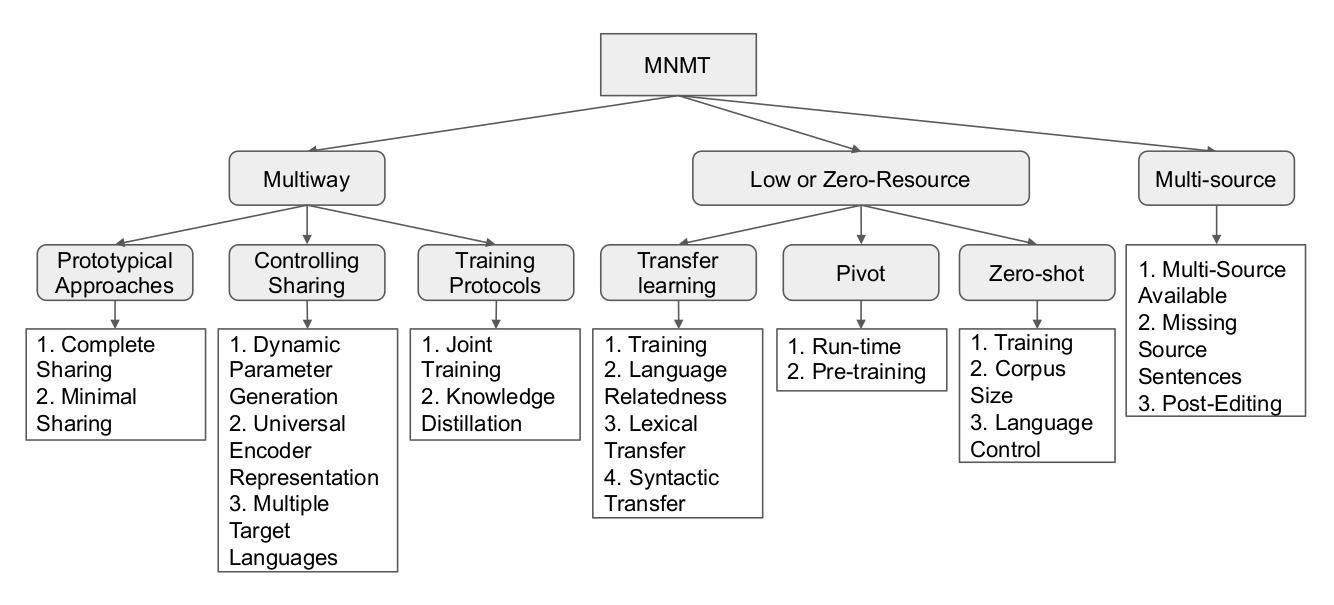
\includegraphics[width=1.0\columnwidth]{../img/dabre_2019_mnmt_categorized.png}
	\end{minipage}\hfill
	\mycaption{%
		MNMT research categorized%
	}{%
		According to resource scenarios and underlying modeling principles.
		By \cite{Dabre2019}
	}
	\label{fig:mnmt_categorized}
\end{figure}


\subsection{Massively multi-lingual machine translation \todo{with complete sharing}}
\label{section:multitarget_theory}

\citet{johnson-etal-2017-googles} proposed a way to build a multi-lingual
machine translation model without any changes to the \emph{Transformer} architecture.
The only change was performed on the input data.
To make the \emph{Transformer} model process multi-lingual data,
they added the desired target language tag to the source sentence.

For example, the following \dir{En}{Cz} sentence pair:
\begin{displayquote}
Hello world! \to{} Ahoj světe!
\end{displayquote}
is modified to:
\begin{displayquote}
\tagto{cs} Hello world! \to{} Ahoj světe!
\end{displayquote}

With the given method, it is possible to produce translations in multiple
languages using the same model just by altering the prepended target language tag.
It was also demonstrated that this method slightly improves translation quality for 
low resource languages when compared to monolingual translation model.

In \cite{aharoni-etal-2019-massively}, models with up to 103 languages were tested.
English centric in-house dataset was used to train \dirmany{En}{Any} and
\dir{$\{$Any$\}$}{En} multilingual models.
The average number of examples per language pair is 940k:
for 13 out of the 102 pairs there were less than one million examples available.

In one of the experiments, they varied the number of languages in the model and measured
the model's performance on the specified set of translation directions.
They started with a 5-to-5 model with English, Arabic, French, Russian, and Ukrainian selected.
Given that the dataset was English-centric, they trained the 5-to-5 model to translate
in \dirmany{En}{Ar, Fr, Ru, Uk} and \dirmanyrev{Ar, Fr, Ru, Uk}{En} directions.
Therefore, name 5-to-5 refers to the model's ability to accept source sentence in 5 languages
and to translate into the same five languages.
For 25-to-25 model they added 20 more randomly selected languages to the 5-to-5 setup.
In all the cases they trained a large Transformer model with 473.7M parameters.
As can be seen in Table \ref{tab:aharoni-2019-performance-drop}, the quality of translation
is significantly worse when a model is trained to translate more languages.


\begin{table}[h!]
\centering
\begin{tabular}{r|cccc}
\toprule
           & En-Ar & En-Fr & En-Ru & En-Uk \\
\midrule
5-to-5     & \textbf{12.42} & \textbf{37.30} & \textbf{24.86} &         16.48  \\
25-to-25   &         11.77  &         36.79  &         23.24  & \textbf{17.17} \\
50-to-50   &         11.65  &         35.83  &         21.95  &         15.32  \\
75-to-75   &         10.69  &         34.35  &         20.70  &         14.59  \\
103-to-103 &         10.25  &         34.42  &         19.90  &         13.89  \\
\bottomrule
\end{tabular}
\mycaption{\acrshort{bleu} scores for translation in one direction
        (part of Table 7 from \citep{aharoni-etal-2019-massively})
	}{
		Model trained on 5-to-5 English centric dataset
		(English to any and any to English) scores 12.42 \acrshort{bleu} for
		English-Arabic test set. Every language from 5 languages
		of 5-to-5 data set is included into 25-to-25 set, as well
		as every language from 25-to-25 data set is included into
		50-to-50 and so forth.
	}
\label{tab:aharoni-2019-performance-drop}
\end{table}


\begin{figure}[h]
	\begin{minipage}{0.48\textwidth}
	\centering
	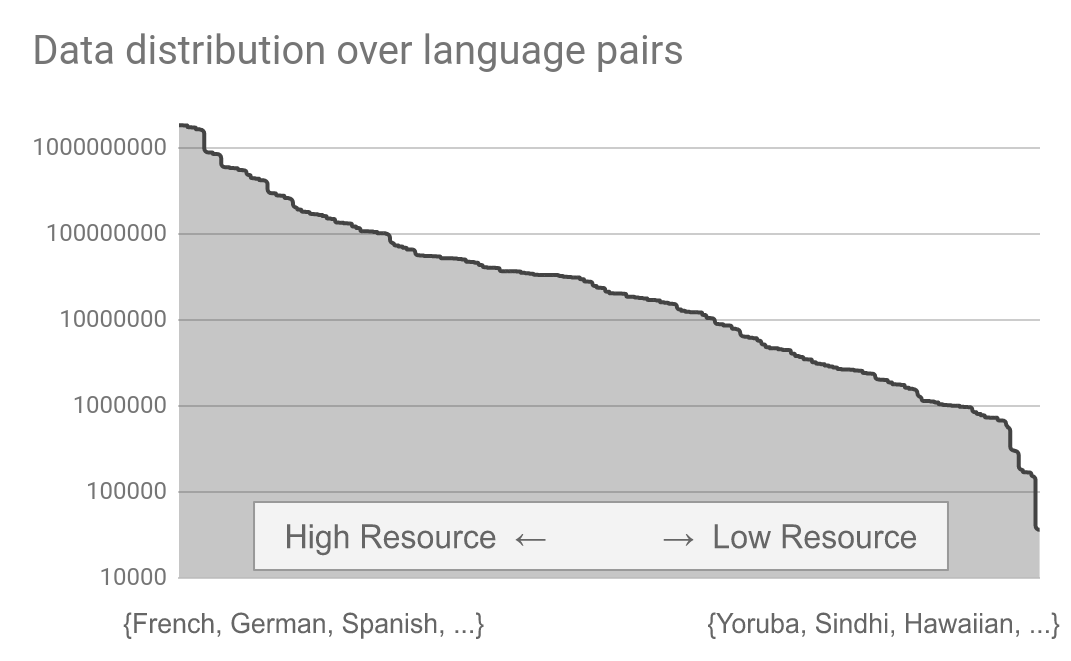
\includegraphics[width=0.9\columnwidth]{../img/arivazhagan-2019-data-distribution.png}
	\end{minipage}\hfill
	%\vspace*{\floatsep}% https://tex.stackexchange.com/q/26521/5764
	\begin{minipage}{0.48\textwidth}
	\centering
	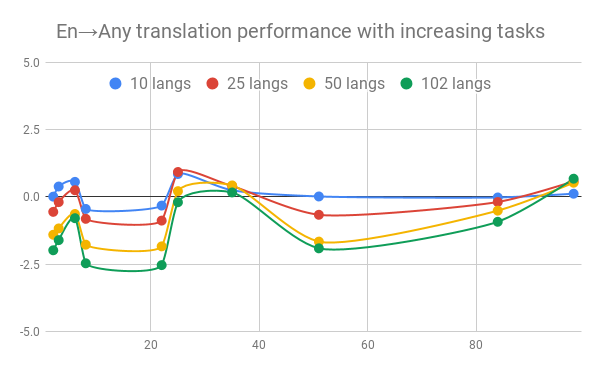
\includegraphics[width=0.9\columnwidth]{../img/arivazhagan-2019-diff-per-n-targets.png}
	\end{minipage}
	\mycaption{
		Tranlsation performance for 102 languages from
		\citet{arivazhagan-2019-mmnmt-in-the-wild}%
	}{
		Axis $X$ is shared between left and right plot.
		On axis $X$ there are languages sorted by amount of training data.
		Left: amount of training data (axis $Y$) for a language.
		Right (best viewed in color): Effect of increasing the number of languages on
		the translation quality. On the axis $X$ the languages are sorted the
		same way as on the left plot. The points visualized are 10 languages
		that are present in all setups
		from En $\leftrightarrow$ 10 to En $\leftrightarrow$ 102.
	}
	\label{fig:arivazhagan-2019-diff-per-n-targets}
\end{figure}


%----------------------------------------------------------------------
\section{Conclusion}

In this chapter we introduced theoretical and historical background for this work.
Firstly, we took a short walk through the history of machine translation.
Then we described the most used type of \acrshort{nmt} models --
self-attention \textit{Transformer} model.
After that we went over the history of translation evaluation in general and the most
used method of automatic evaluation -- \acrshort{bleu} -- in particular.
In the end, multi-lingual neural machine translation was reviewed
with more detailed view into `complete sharing' scheme.
